\chapter{Knowledge to be gained from \textit{The Visual Display of Quantitative Information} facing CIRDLES' new ploting library.}

\section{Introduction}
Topsoil is the latest projet from the CIRDLES' lab. It allow geochronologists to plot various graphs needed for the analysis of aliquots. This software is based on the JavaFX library which gives to Java the ability to display user interfaces.

The first and current version of Topsoil is using the ploting abilities of JavaFX. But as we copied and rewrite part of these to make them fit our needs, we quickly realized that they had too much flaws to be a long term solution.
 Being a long term solution is one of Topsoil's objective. We needed another library to plot our graphic.

After a long and laborious search, John did not found one that could plot graphics for us. The solutions were either too specific, not well-designed enough or not compatible with JavaFX. From that moment on, it became clear that we needed to create our own graphic library. 

Although designing, coding and maintaining this kind of library is a lot of work, the result will be worth the effort.
 Since it is still preferable that the team document itself before starting a project of this scale,
 I've red \textit{The Visual Display of Quantitive Information} by Edward Tufte and gathered some informations, presented in this rapport.
\\

This document is structured in three parts : 
\begin{itemize}
\item First of all, a very brief summary of the book will be given, allowing the reader to feel its tone.
\item Then charts that the library should be able to produce and their interesting particularities will be shown.
\item Finally, some of Tufte's rules for making good diagrams that the library should enforce or encourage to enforce will be listed. 
\end{itemize}
\emph{Please note that the recommendations contained in that report should not be exactly followed right away. They are useful to see the big picture.}%To be rephrased




\section{A quick summary of this book}
This book is a manifesto. It assert that charts are powerful tools of communication, explain why and how to make great graphics.
Along the book, Tufte find regrettable the underusage of plots in many kinds of publications, like textbooks, papers or journals. He also list a few reason of this underusage.

In the first part of his book, great graphs are listed. Then, errors that cause the integrity of the graph are given. Tufte describe the separation of graph and text, and the unfortunate simplicity of most of today's chart.
Finally, a set of rules that make great diagrams are given.




\section{A list of graphic}
Our library should support a lot of type of graphics, and in that regard, the team should know a wide range of them. To expend that knowledge, a number of chart along with the features needed in order to support them will be given here.

\subsection{Data Map chart}
Laying out data on a map can with no doubt carry enormous volume of data and have multiple reading levels.

%Complexe line representing the sea.
\centerline{
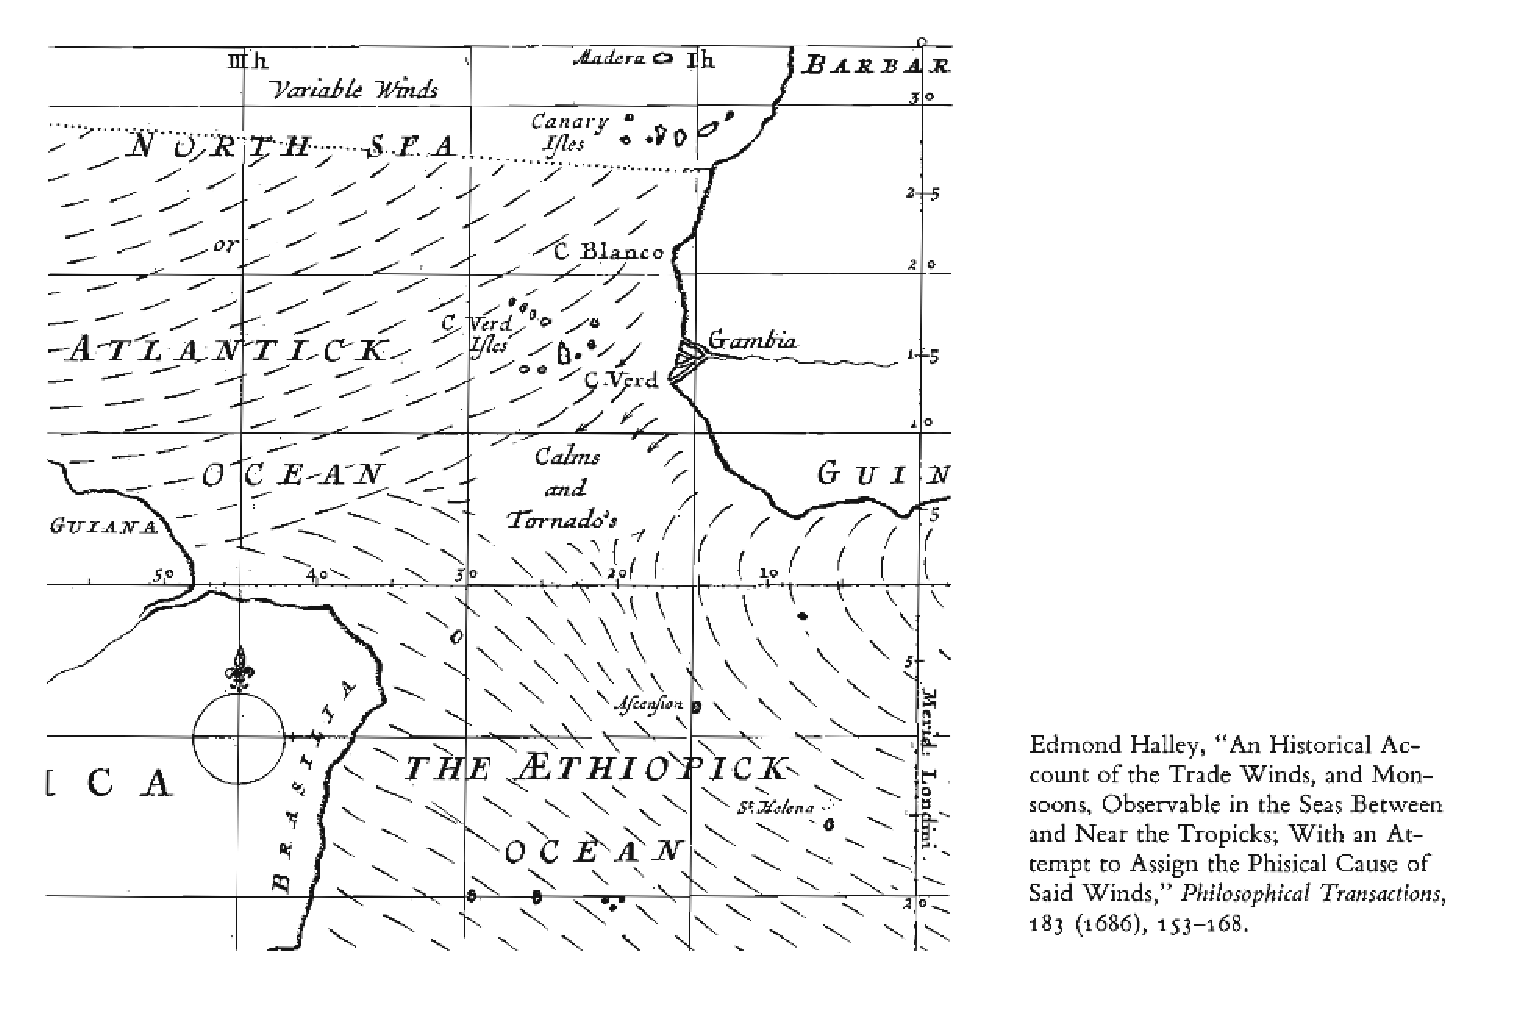
\includegraphics[width=07cm]{./illustrations/annexes/carte_courants.eps}
}
Our library would have the ability to plot this if it could fill up its graph's background with a map
 including name of landmarks
\footnote{Further research hint : interoperable map format or map plotting libraries}.
 The possibility to add symbols of all kind, from a single point on a city to complex shape is also needed. 

%Cancer map
\centerline{
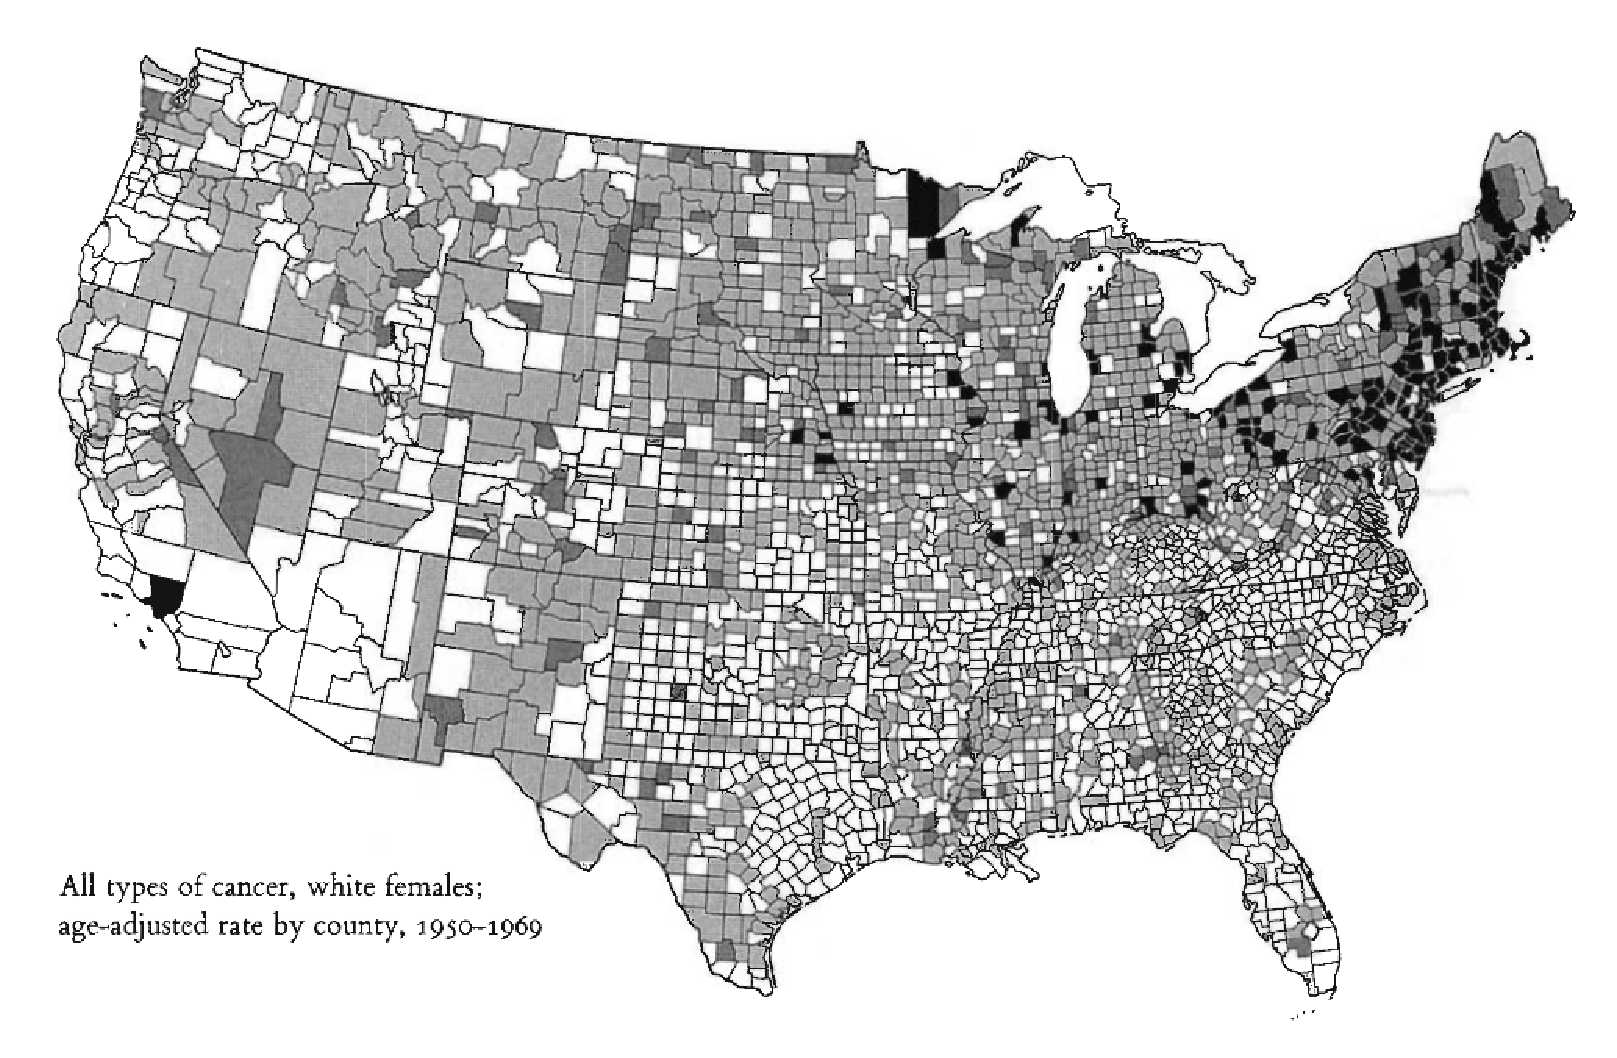
\includegraphics[width=07cm]{./illustrations/annexes/carte_cancer.eps}
}
An other important feature to consider is binding data to zones on background's map, as seen of this chart.

%French export
\centerline{
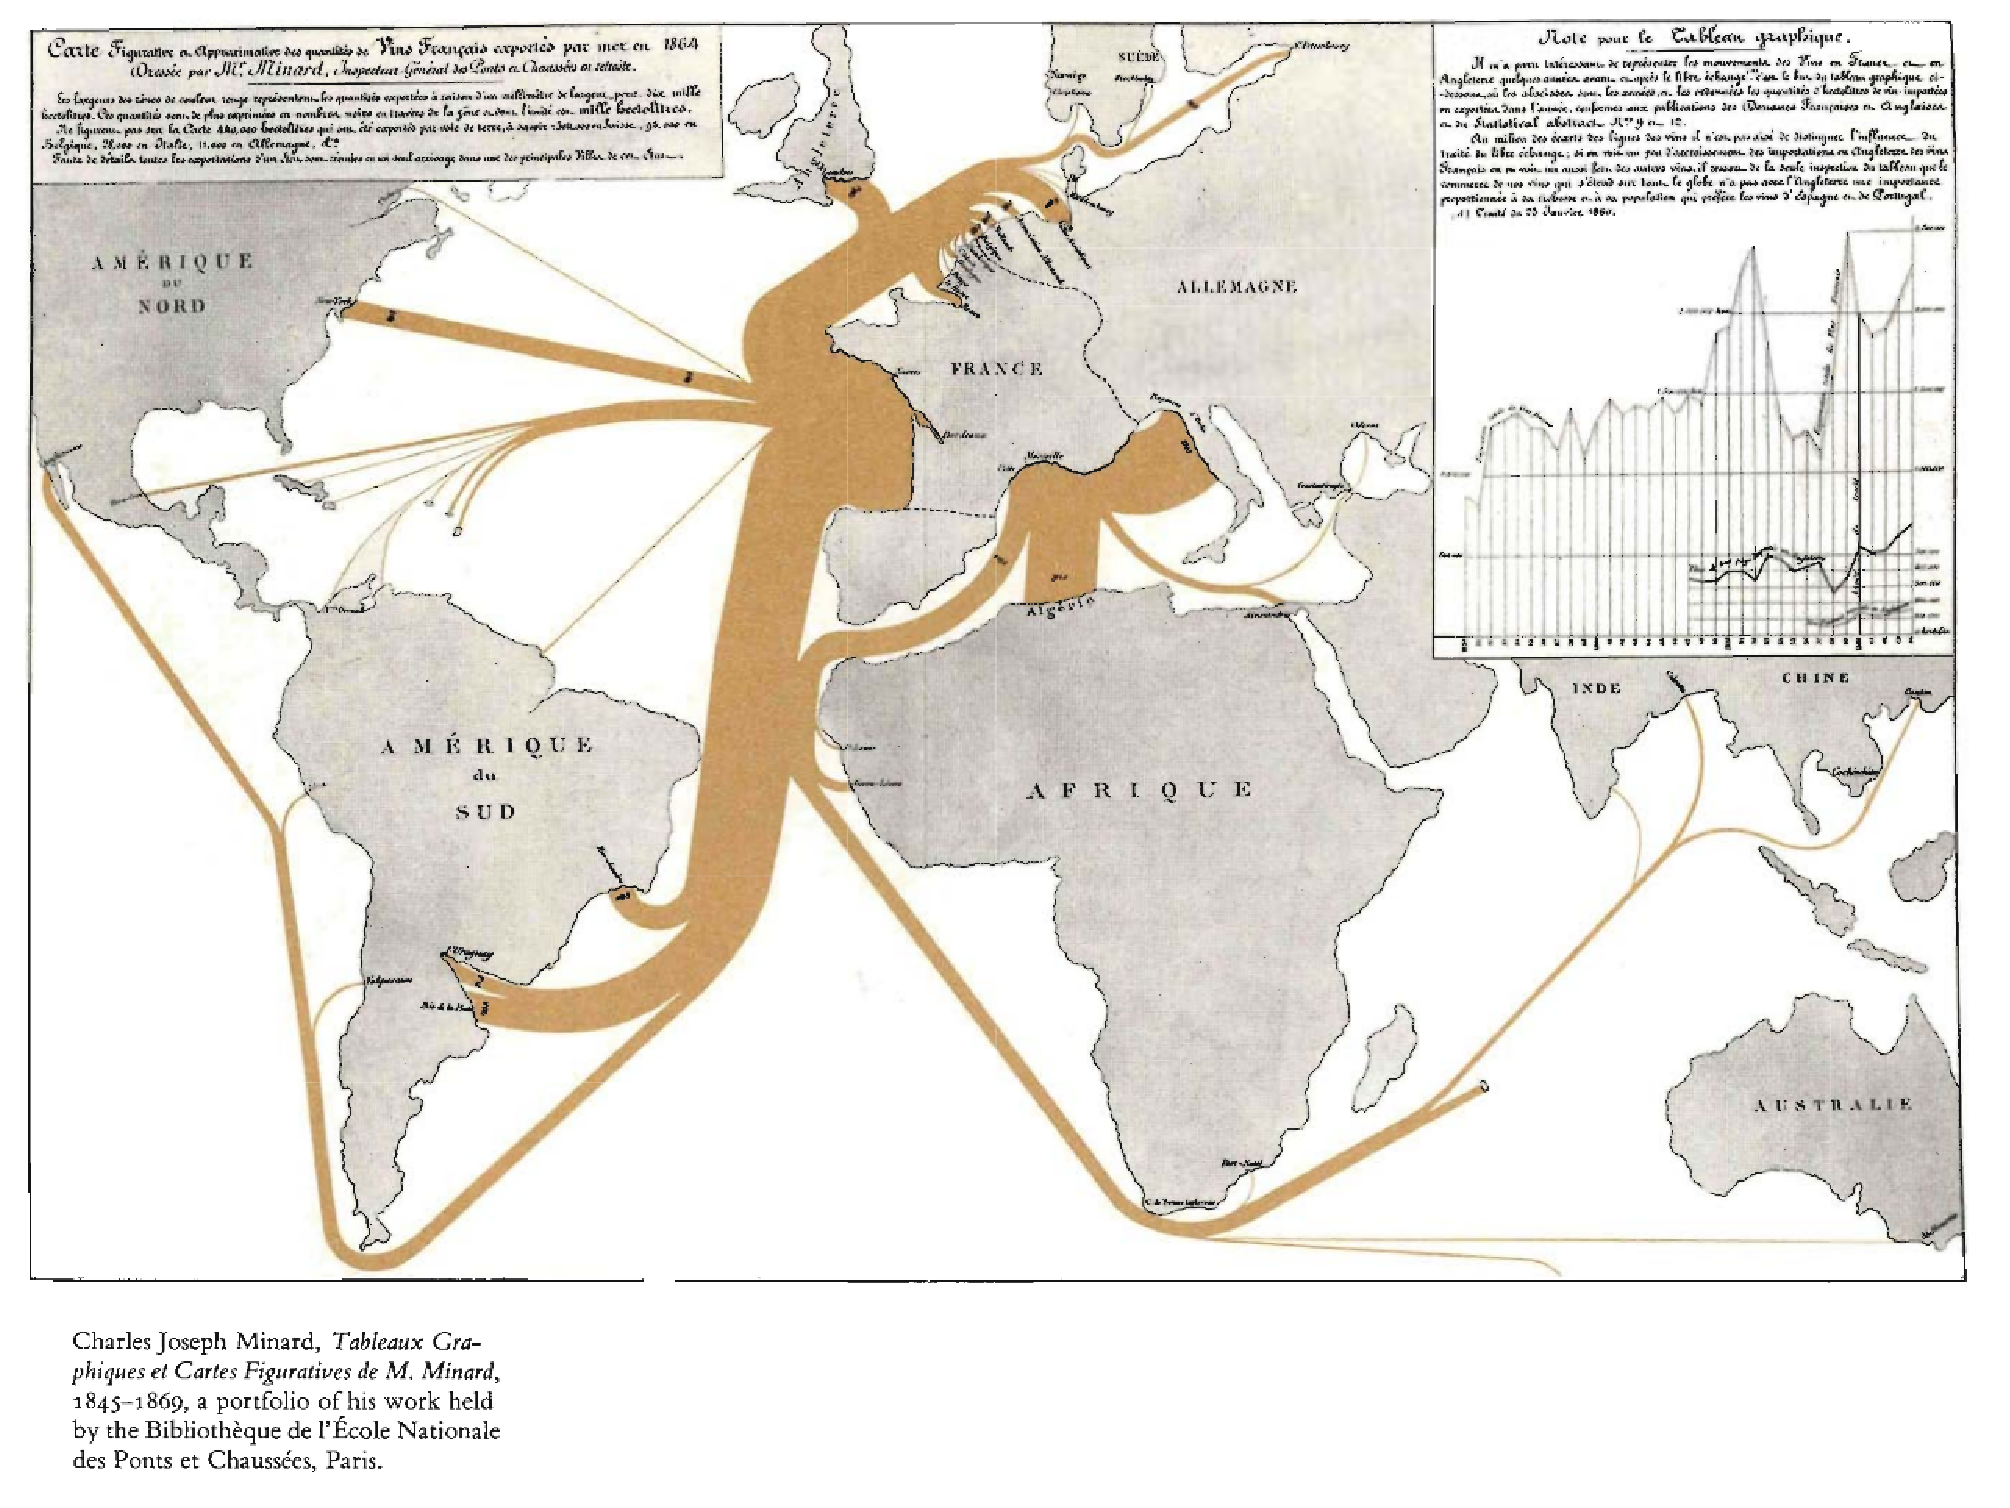
\includegraphics[width=10cm]{./illustrations/annexes/carte_exports.eps}
}
Several layers of the map have to be considered to render thoses lines. The informations passed to draw them are :
\begin{itemize}
\item Position of the begining
\item Position of the end
\item A quantity
\end{itemize}
These are the two reasons why the map have to be considered when plotting these lines :
\begin{itemize}
\item The line is drawn from its begining to its end, \emph{bypassing earth}.
\item The begining and the end must fit closely the earth. 
\end{itemize}

\subsection{Time-Space chart}
%NY City Weather
\centerline{
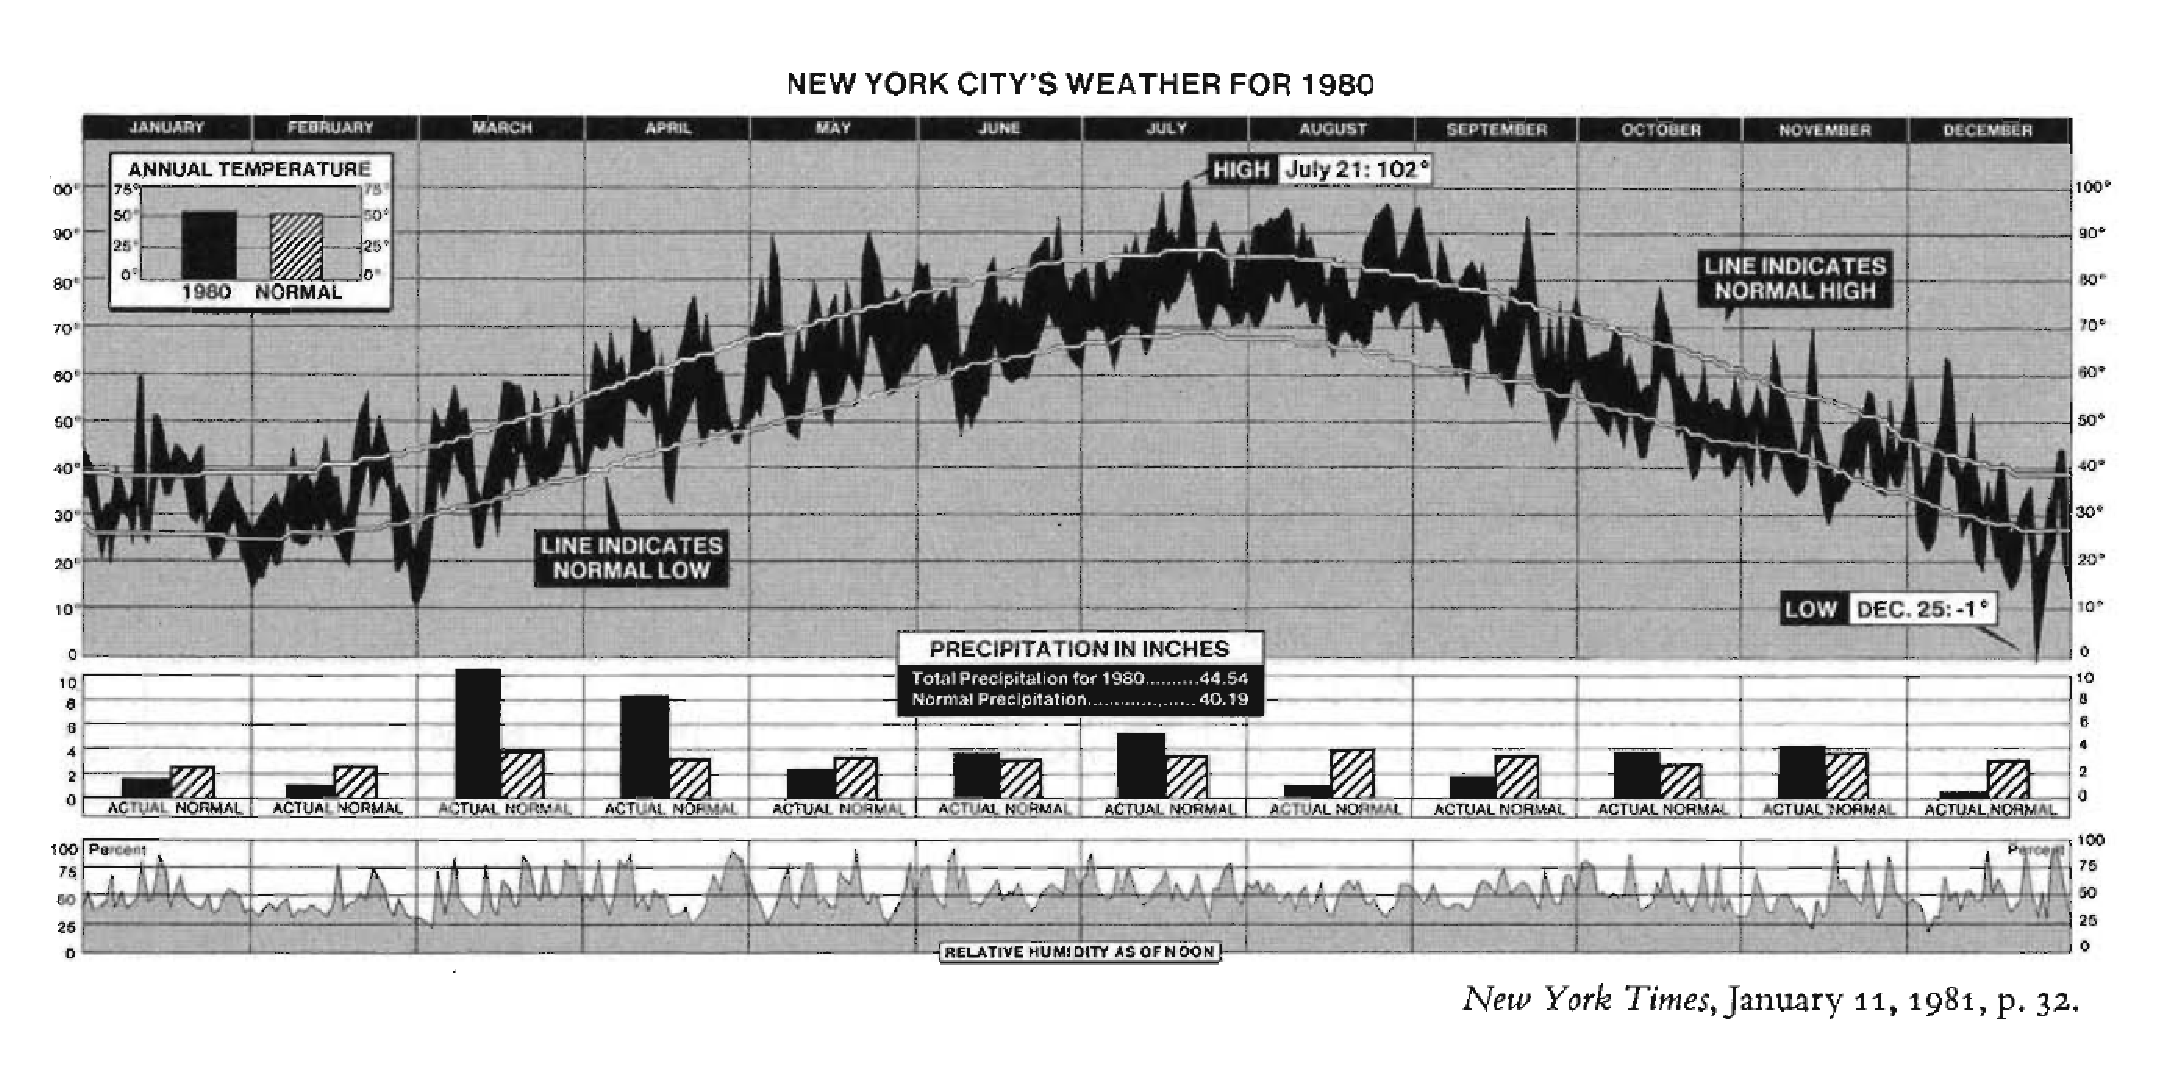
\includegraphics[width=10cm]{./illustrations/annexes/temps_nymeteo.eps}
}
Several \emph{important} informations can be gained from that plot.

First, notice the indications pointing on the main curve (like \emph{"Line indicate the normal low"}). Tufte love them.
 They point either to a data point, to a serie, or to nothing (in that case they just have a position on the graph).

Secondly, notice that the temperature axis is printed twice, on the two sides of the graph.

Thirdly, there is one subgraph drawn for each month representing the difference between the actual precipitation and the normal.
 The idea of series of subgraph is to be considered.

Last, but not least : the several pieces of data are linked to the same x-axis but to different y-axis.

%Playfair : "Sharing at one wiew the Price of Quarter of Wheat ...
\centerline{
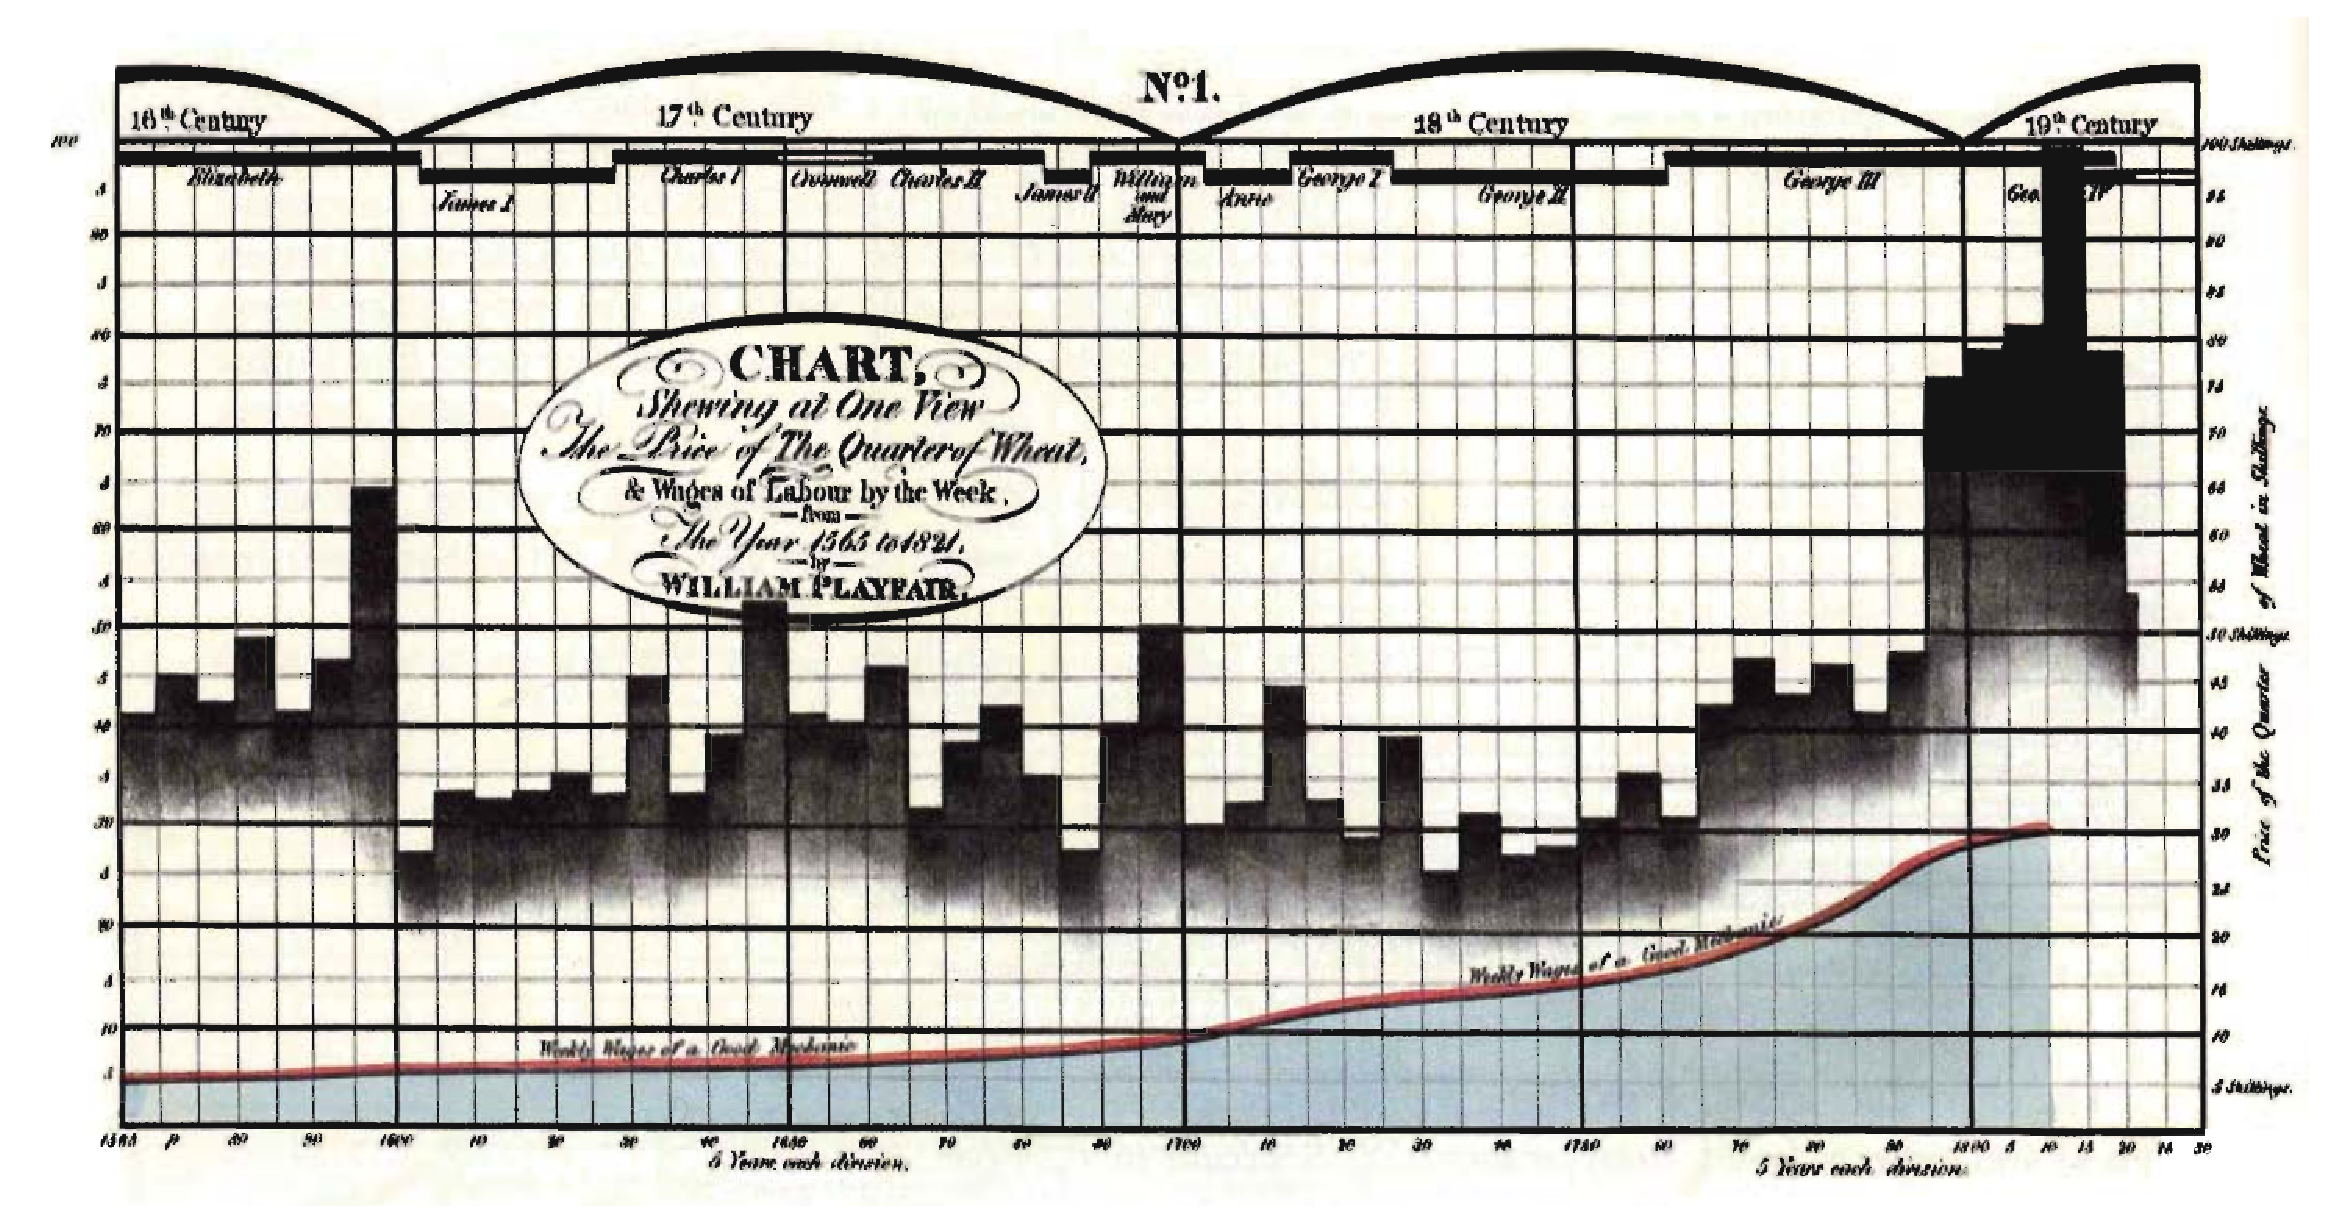
\includegraphics[width=10cm]{./illustrations/annexes/temps_ble.eps}
}
Concerning this diagram, I cannot think of more than one axis of reflection for now. There are two sets of data that have there own space, making the plot more readable. Maybe we could arrange plot of data to be aware of their sibblings, or make the PlotArea smarter when it is outlining two set of data.

%http://worldtracker.org/media/library/Science/Science%20Magazine/science%20magazine%201981-1982/Science%201981-1982/root/data/Science_1981-1982/pdf/1982_v216_n4550/p4550_1086.pdf

\subsection{Time-Space chart}
%Teh Napoleon Chart
\centerline{
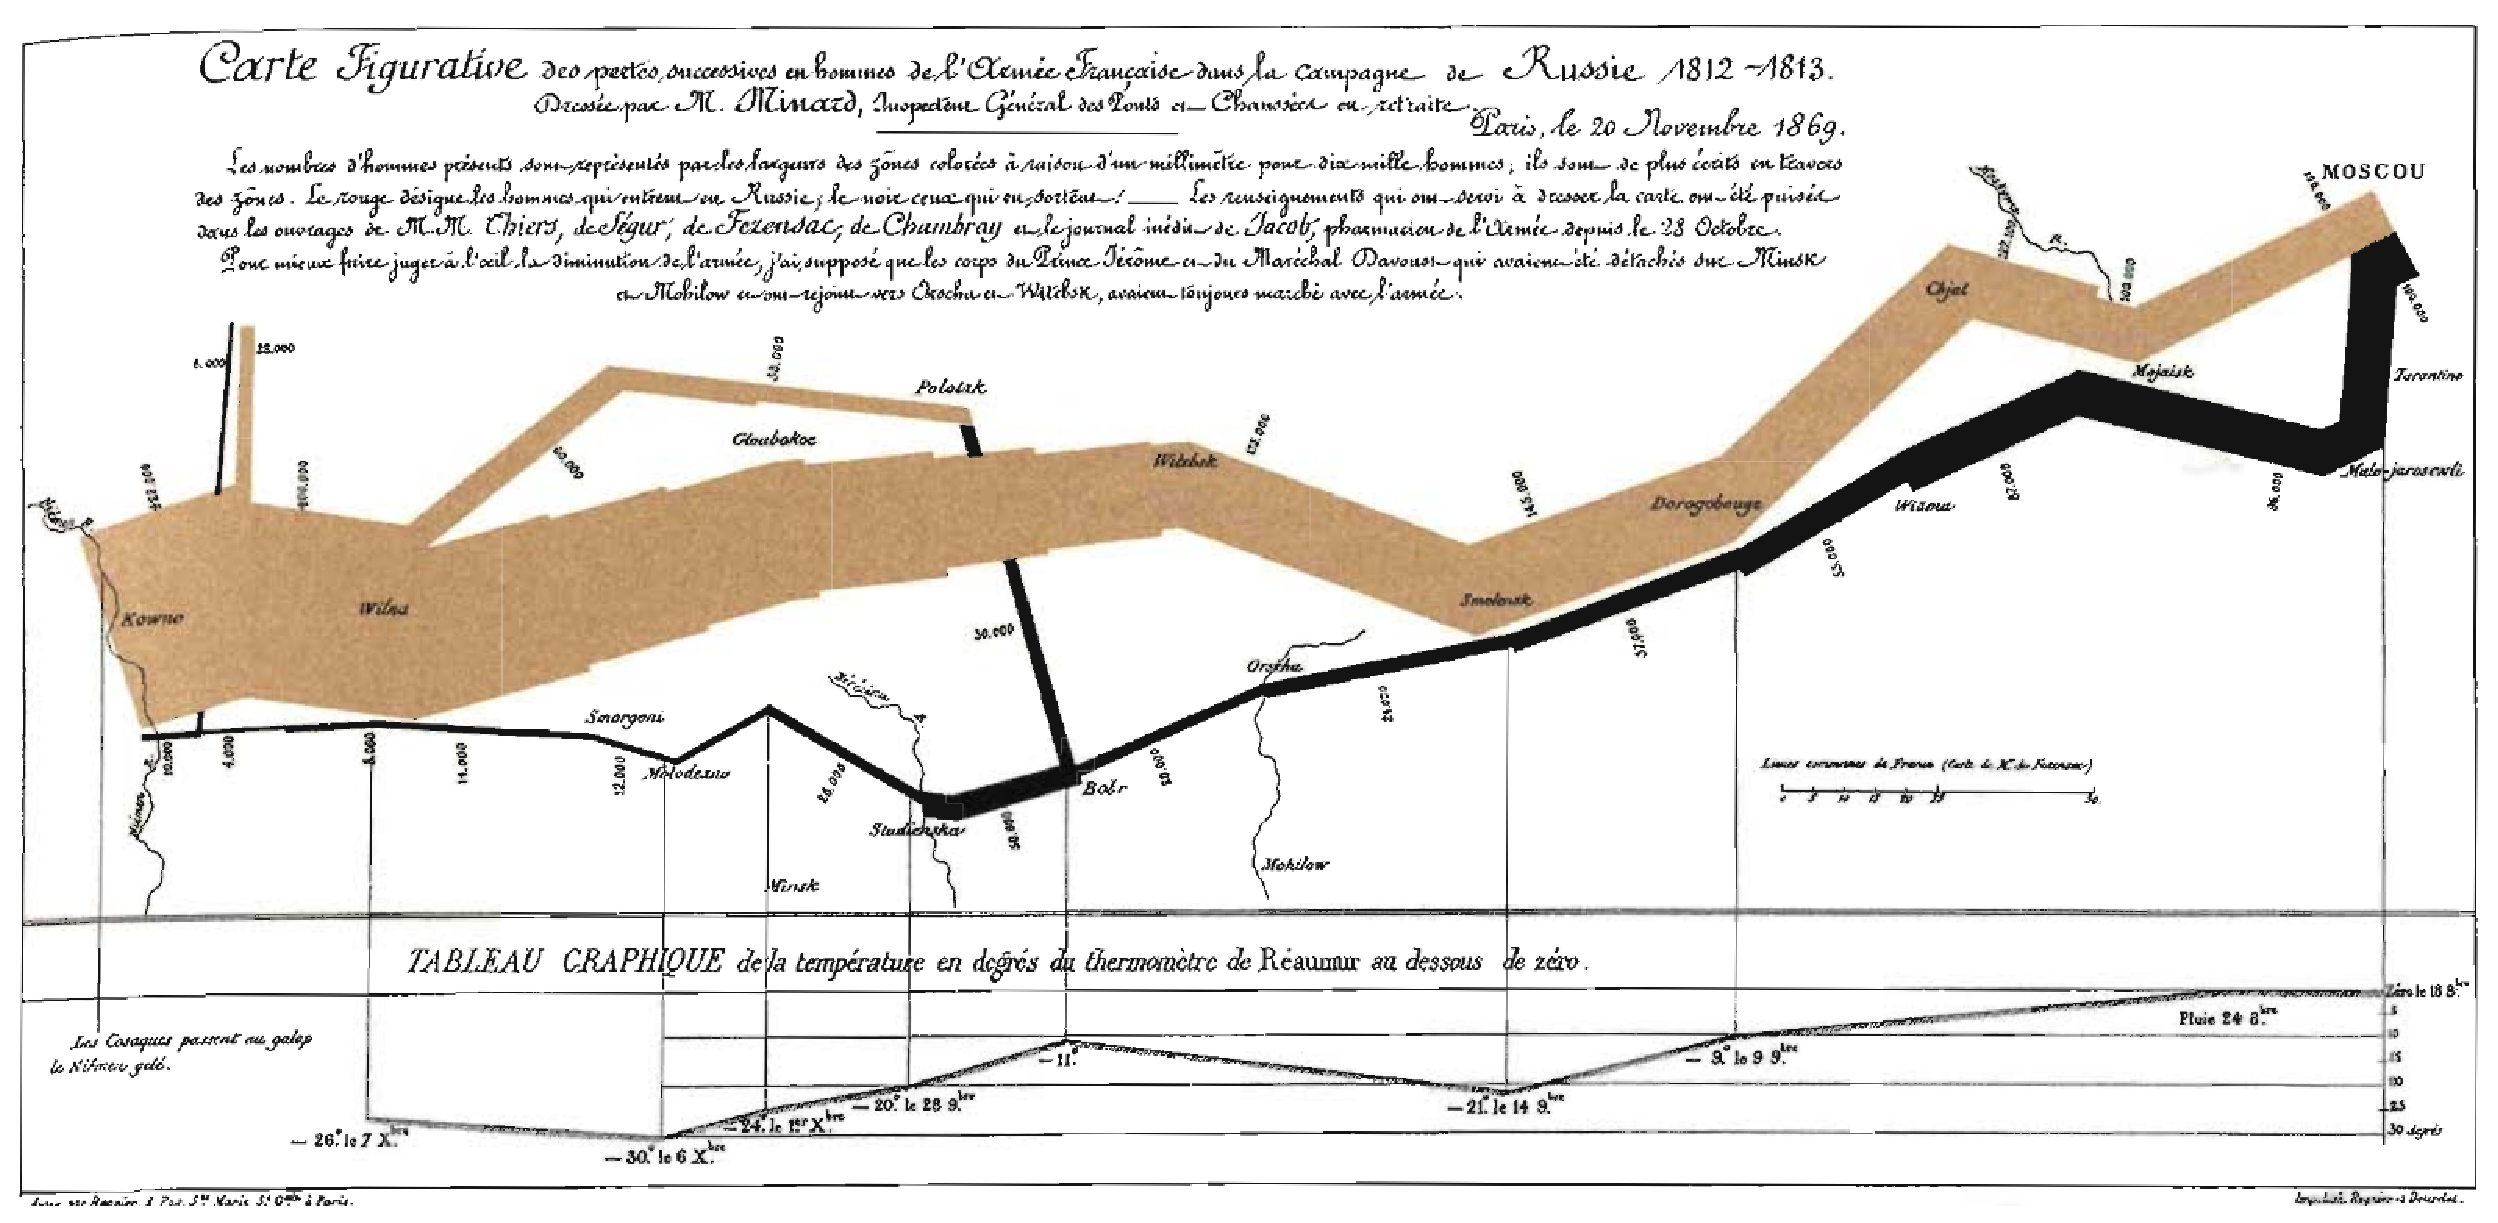
\includegraphics[width=10cm]{./illustrations/annexes/tempscarte_napoleon.eps}
}
The very interesting construction of the diagram is here made in two times.

First, the path of Napoleon's army in russia. The following data is given 
\footnote{Excluding the travel direction of the army that give the color, not relevant to my pointin this context}
 for each step to draw it :
\begin{itemize}
\item The location of the step
\item The number of soldier that was at that moment in the army
\item The date 
\end{itemize}

The plot of a serie of data is made not only of the representation of its data-points, but also of the representation of surrounding informations.
 For exemple, here, if we ploted all the plot one at the time, the location would be drawn, but not the path between two of those location.

Second and bellow, the temperature of each steps.
 The y-axis of this part is simply representing the temperatures.
 The x-axis on the other hand is ``the step'', and is the plot of Napoleon's army path. The plot is an axis. This is a very interesting use case.

\section{Several principles that make a good plot}
Edward Tufte give in his book several principles that make a good chart. For the moment, I do not certify that all of those rules will be of some help for our work. I still think the team should be aware of their existence.

There are two sort of rules : \begin{itemize}
\item Those which avoid misleading diagrams  
\item Those which allow a better presentation of the plot
\end{itemize}

\subsection{Keeping graphical integrity} 
Tufte put together five rules that ensure the graphic's integrity.

\hrulefill

\begin{quote}
The representation of numbers, as physically measured on the surface of the graphic itself, should be directly proportional to the numerical quantities represented.
\end{quote}
This is not always the case and lead to misinformation of the uncareful viewer. Tufte invented a unit representing how much the diagram is lying : the Lie Factor.

$$\text{Lie Factor} = \frac{\text{size of effect shown in graphic}}{\text{size of effect in data}}$$

A quick exemple of the Lie Factor :

%Image of the Fuel Economy Standards for auto
\centerline{
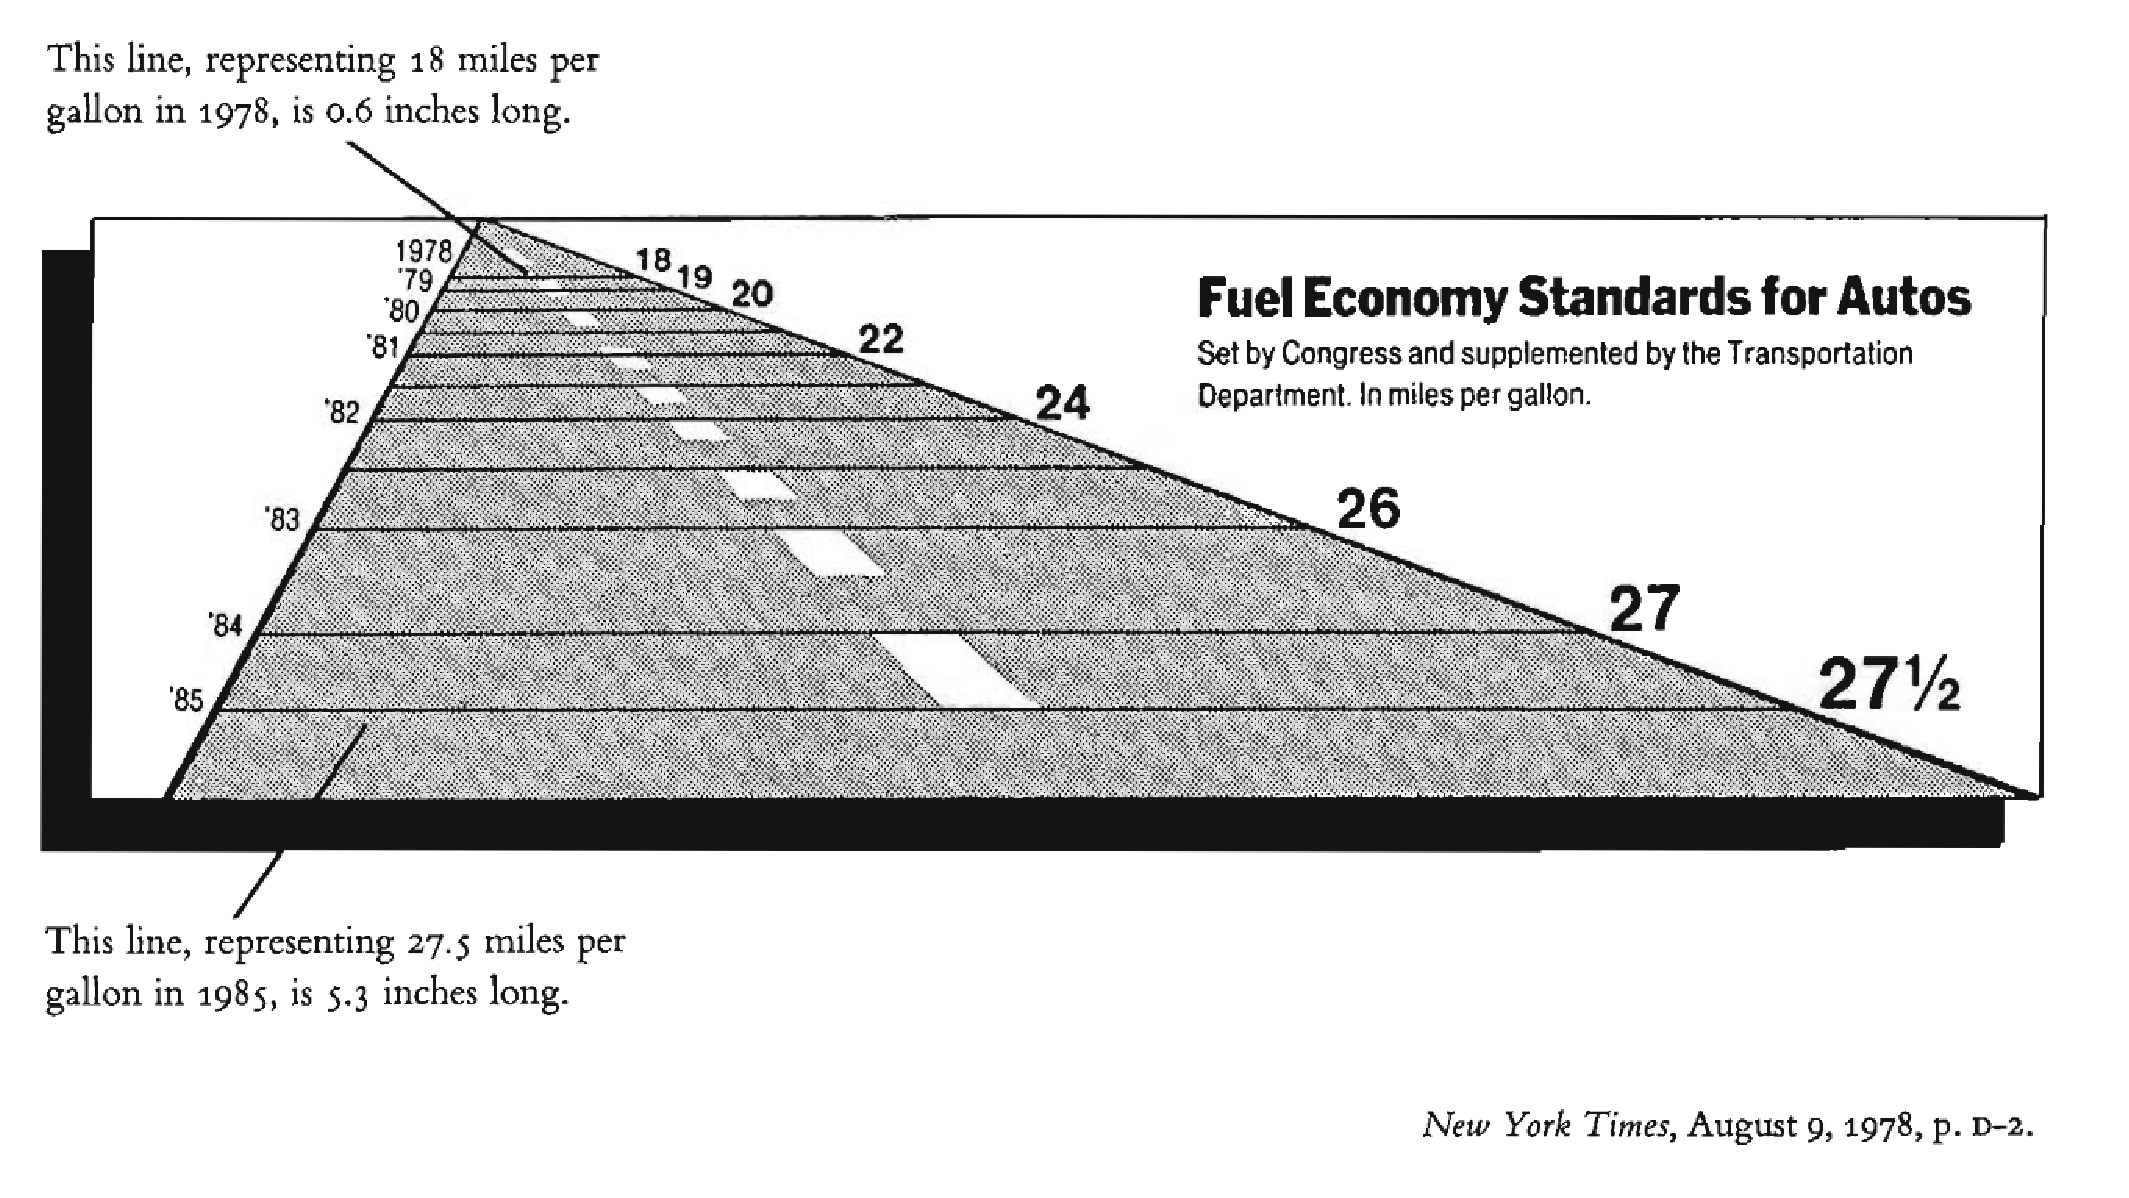
\includegraphics[width=07cm]{./illustrations/annexes/temps_fuel.eps}
}

\begin{itemize}
\item The increase between 18 and 27 is \emph{53\%}
\item The increase between 0.6 inch and 5.3 inch, the size of the two side of the road is \emph{783\%}
\end{itemize}

The lie factor is  : $\frac{783}{53} = 14.8$ 

\hrulefill

\begin{quote}
Clear detailed and thorough labeling should be used to defeat distortion and ambiguity. Write out explanations of the data on the graphic itself
\end{quote}

As said before, the library should provide a way to add text, possibly linked to data, or the serie of data.

\hrulefill

\begin{quote}
Show data variation, not design variation.
\end{quote}

The unit on the axis should never change.
 On some of the book's graphics' x-axis, the section between tick represent a year.
Then it suddenly switch to one month.
 It is not may obvious and the unfocused viewer suddenly see a drop in the data. 

The aspect ratio of the graphic also matters. A graphic taller than wide can depict a normal situation as skyrocketing.

\hrulefill

\begin{quote}
In time-series displays of money, deflated and standardized units of monetary measurement are nearly always better than nominal unit
\end{quote}

\hrulefill

\begin{quote}
The number of information-carrying (variable) dimensions depicted should not exceed the number of dimensions in the data.
\end{quote}

There are considerable ambiguities in how people percieve a two-dimensional surfaces, and making the area proportional to the data is a perilous task. For a data made of a single number, a single dimension shape, like a line, is better.

\hrulefill

\begin{quote}
Graphic must not quote data out of their context
\end{quote}

%Image of the nazi thingy
\centerline{
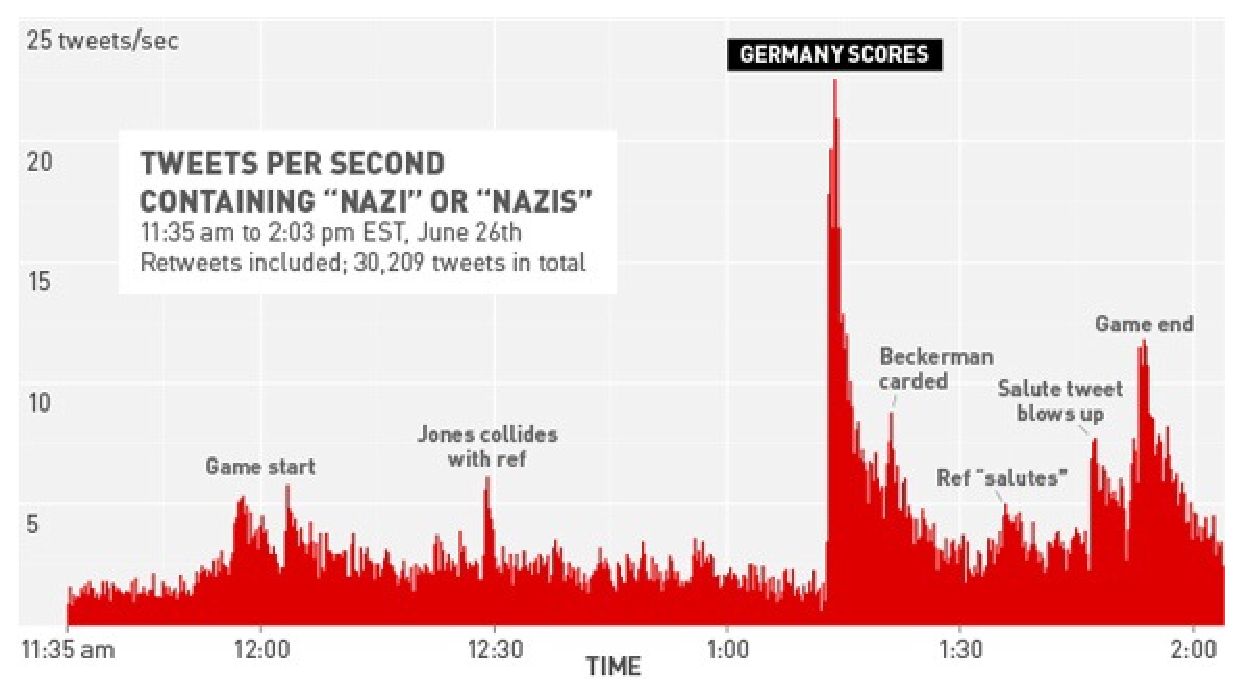
\includegraphics[width=07cm]{./illustrations/annexes/temps_nazi.eps}
}
This image shows us the number of time by seconds the words "nazi" and "nazies" were tweeted during the USA vs. Germany match. It rose from 5 to 25 when Germany scored.

On that graphic, it seems to be a major event. But none of the data shows us how many time the word is tweeted during the rest of the year.
 It could be a lot more than that or a lot less, and we have no way to know.









\subsection{Building clearer graphic}
\begin{quote}
Above all else, show the data
\end{quote}

Tufte believe that most of the ink (or pixels in our case) of the chart should be used to draw the data. He even invented another ratio to measure how much the graphic was clogued up by unuseful drawings.

$$\text{Data-ink ratio} = \frac{\text{data-ink}}{\text{total ink used to print the graphic}}$$

The data ink comprise nothing exept the object representing the data. This means that the objects allowing the representation to make sense (axis, texts) are not included. 

This is why the data-ink ratio must most of the time never be one, but should stay near one.

A grid too precise, axis overloaded, unrelated drawing : all of those block a graphic, preventing it to deliver correctly the data.

%Image d'un histogramme
\centerline{
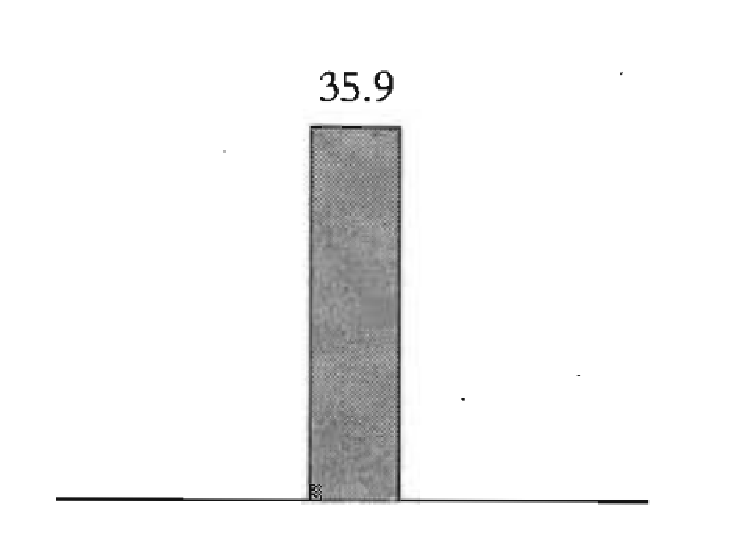
\includegraphics[width=07cm]{./illustrations/annexes/histogramme.eps}
}

Representing the data multiples time is also orverloading a chart. On this bar, the number ``35.9'' is represented in 6 ways :
\begin{itemize}
\item Height of the left line
\item Height of the right line
\item Height of the shading
\item Height of the top line
\item Position of the text
\item Text itself
\end{itemize}

This is ink lost and chart complexified for nothing. Remember, it's like in a movie : You don't need three shots of a women saying one sentence if one is as efficient. 
 And you don't need to move around her unless you have a good reason. 
 Damn you, Michael Bay.

 A chart creator should always try to represent one information with less ink as possible.
 One hint, in order to achieve this : Symmetry always represent the data twice.

%Image : Moire
\centerline{
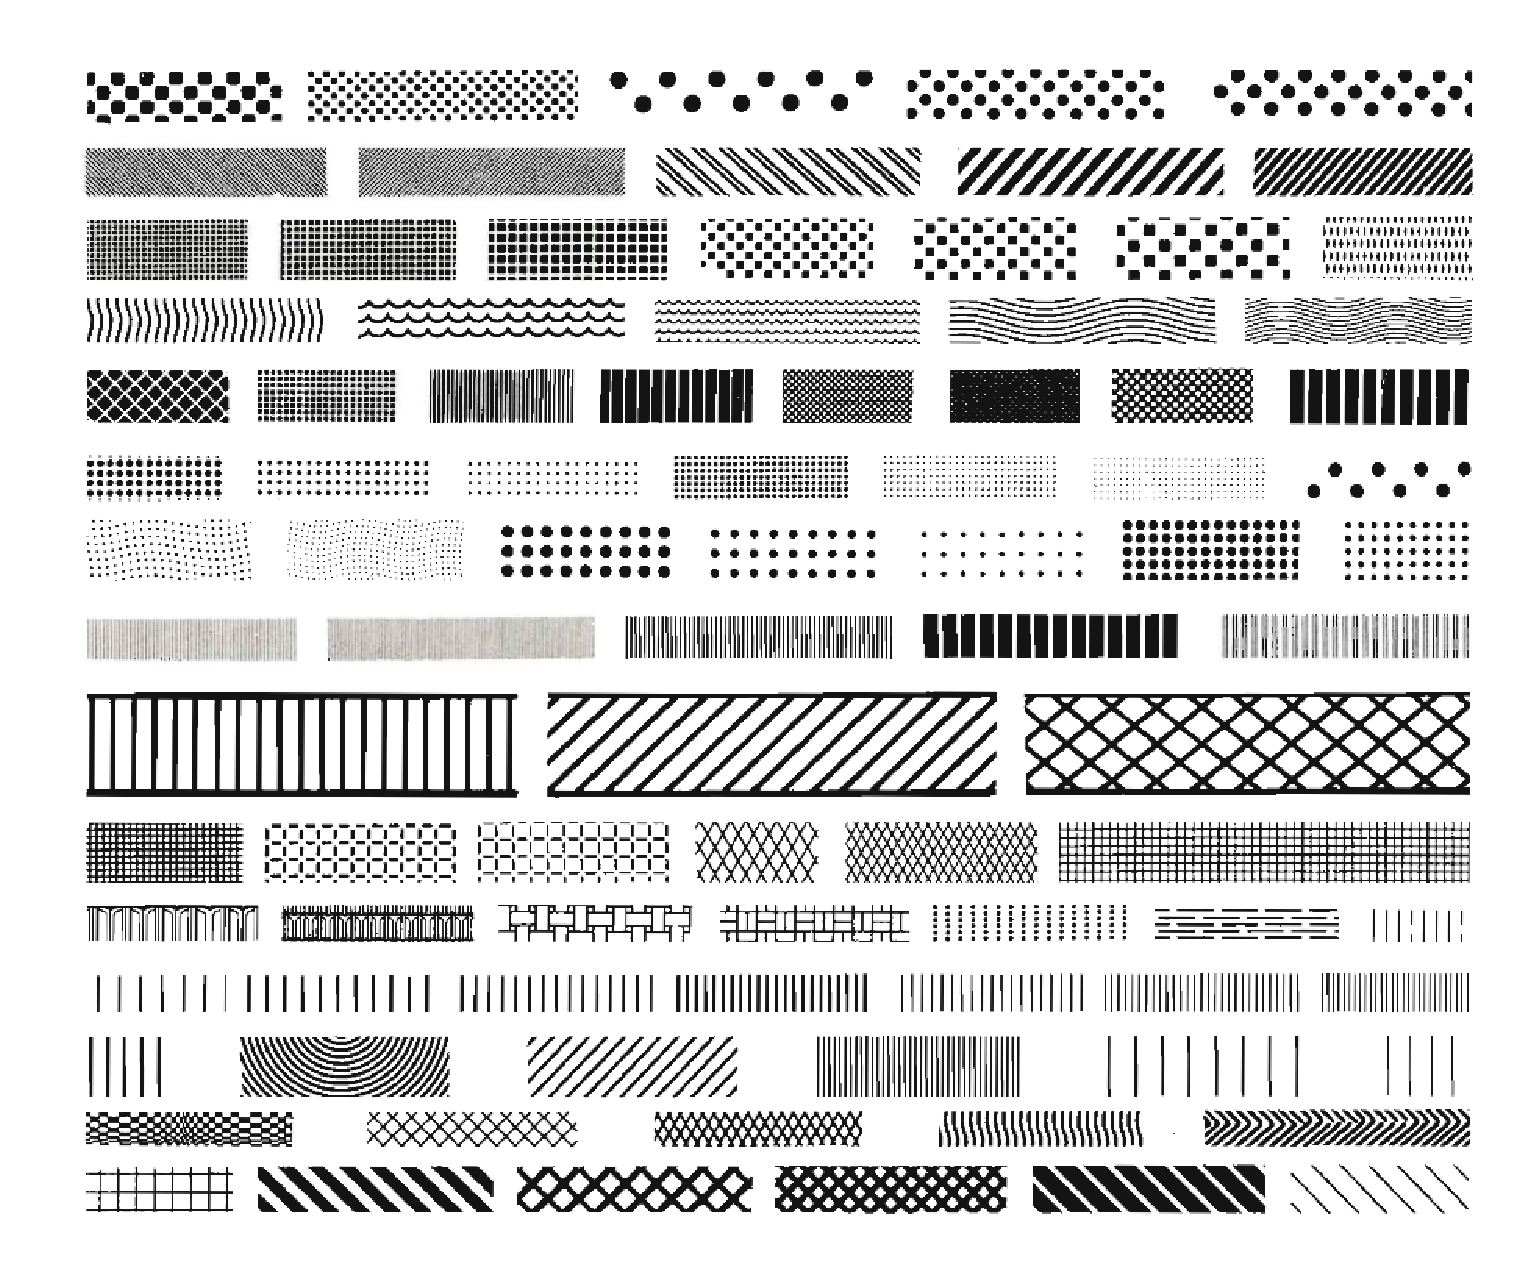
\includegraphics[width=07cm]{./illustrations/annexes/moires.eps}
}
Above, you will find several type of moiré effects. Printing them on a chart make it less clear and less attractive.
 Considered when computer ploting was created as a modern effect, it has ever since plagued chart. The library shall not encourage this trend.

The grid is also an element that can obfuscate a chart : It compete with the data and is not often necessary.
 It can be useful only when the graph serve as a look-up table, but even then, it shall be lighter than the data and remain in the background. 

In those cases, the white grid is a good idea. The white grid is printed by erasing part of the data where a grid should cross it. Here's an exemple :
%The white grid shall go here
\centerline{
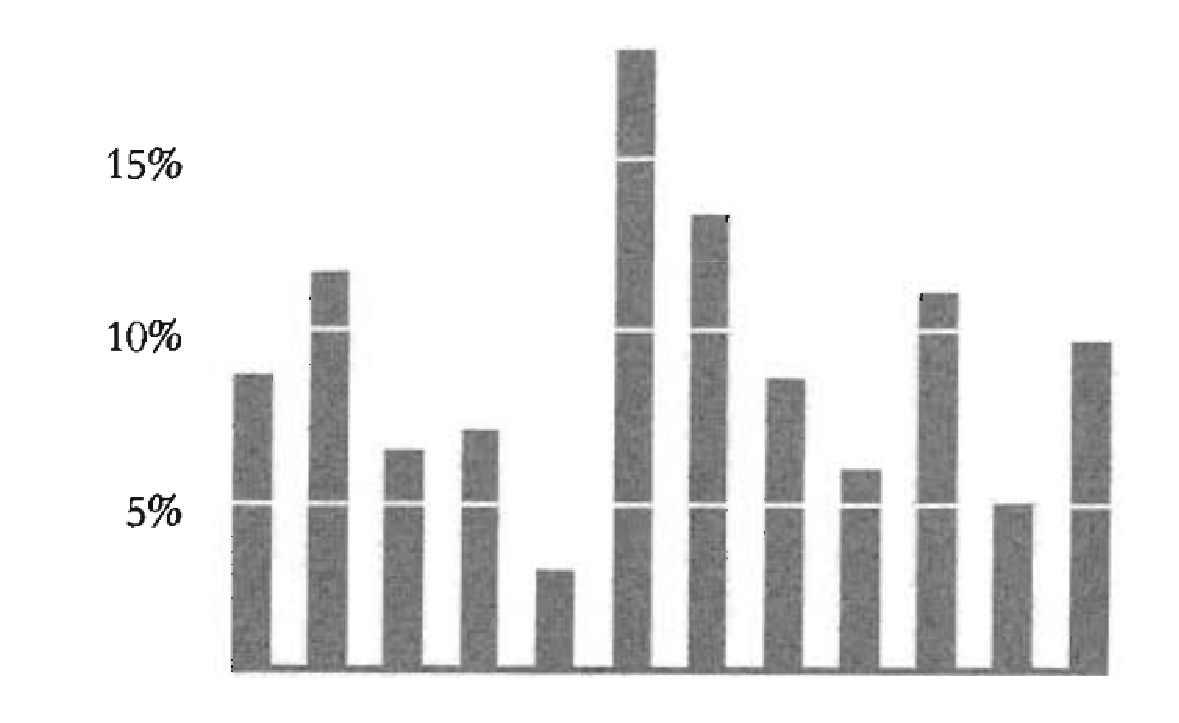
\includegraphics[width=07cm]{./illustrations/annexes/grilleblanche.eps}
}

The axis are also almost never used at their best. By erasing or moving part of it, we can show more data : 

%Image : Chart p.132
\centerline{
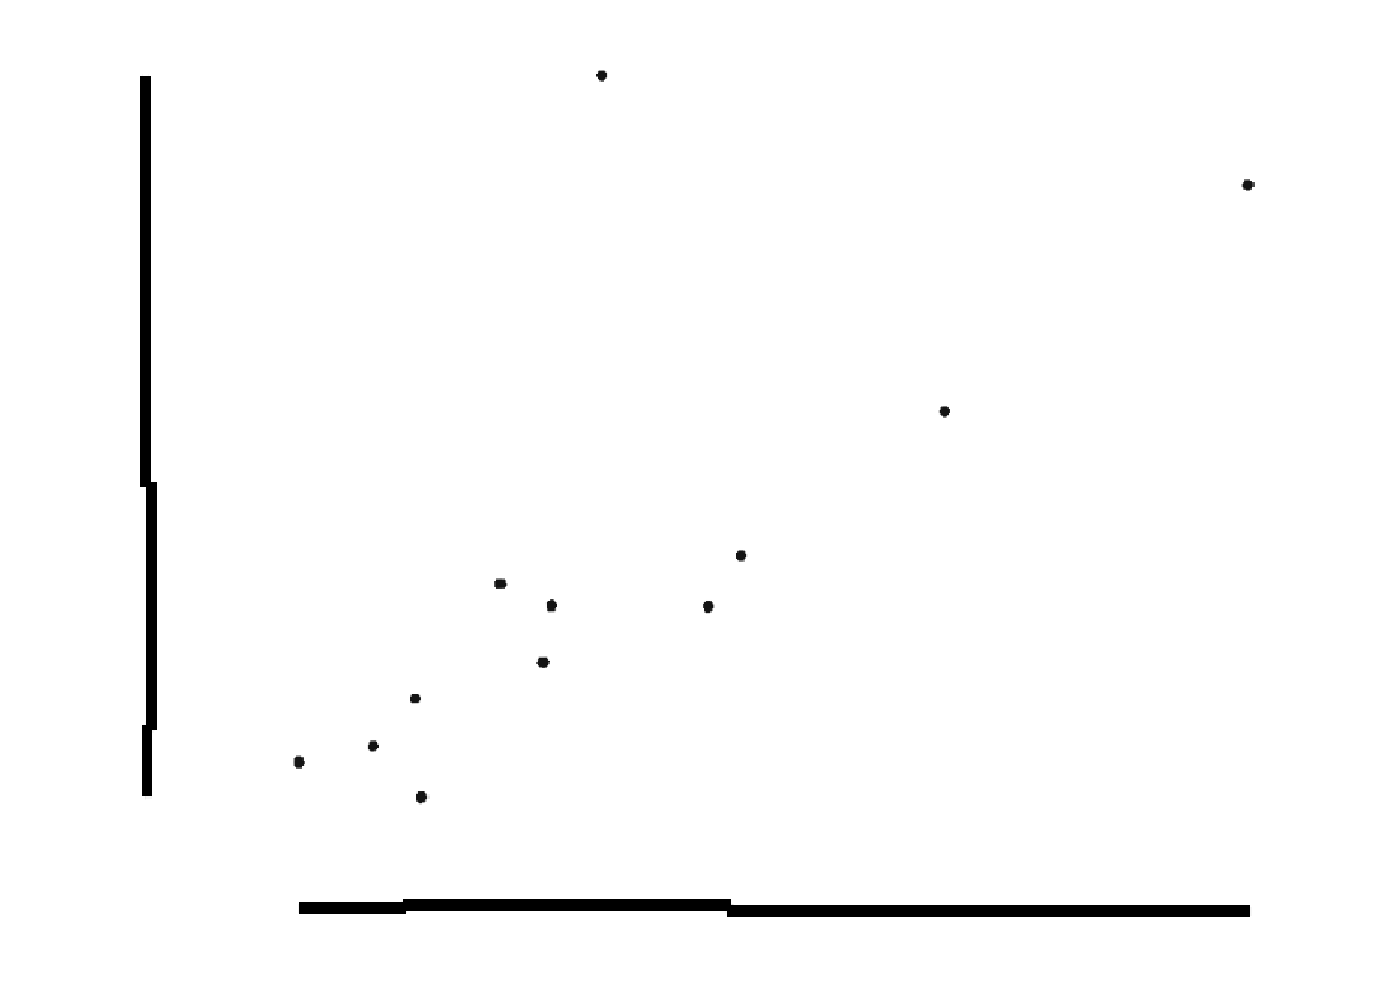
\includegraphics[width=07cm]{./illustrations/annexes/axesmodernes.eps}
}

On this chart, ten numbers have been added to the set of data : 
\begin{itemize}
\item the minimum and maximum are shown by begin and ending the axis at their value
\item the shifted part of the axis represent three quartil : lower, upper
\item the erased portion in the shifted part show the median quartil
\end{itemize}
Since these value are shown on the two axis, we have $5*2$ values that have been added.

An axis can also show the marginal distribution of each variables :

%Image : image p.133
\centerline{
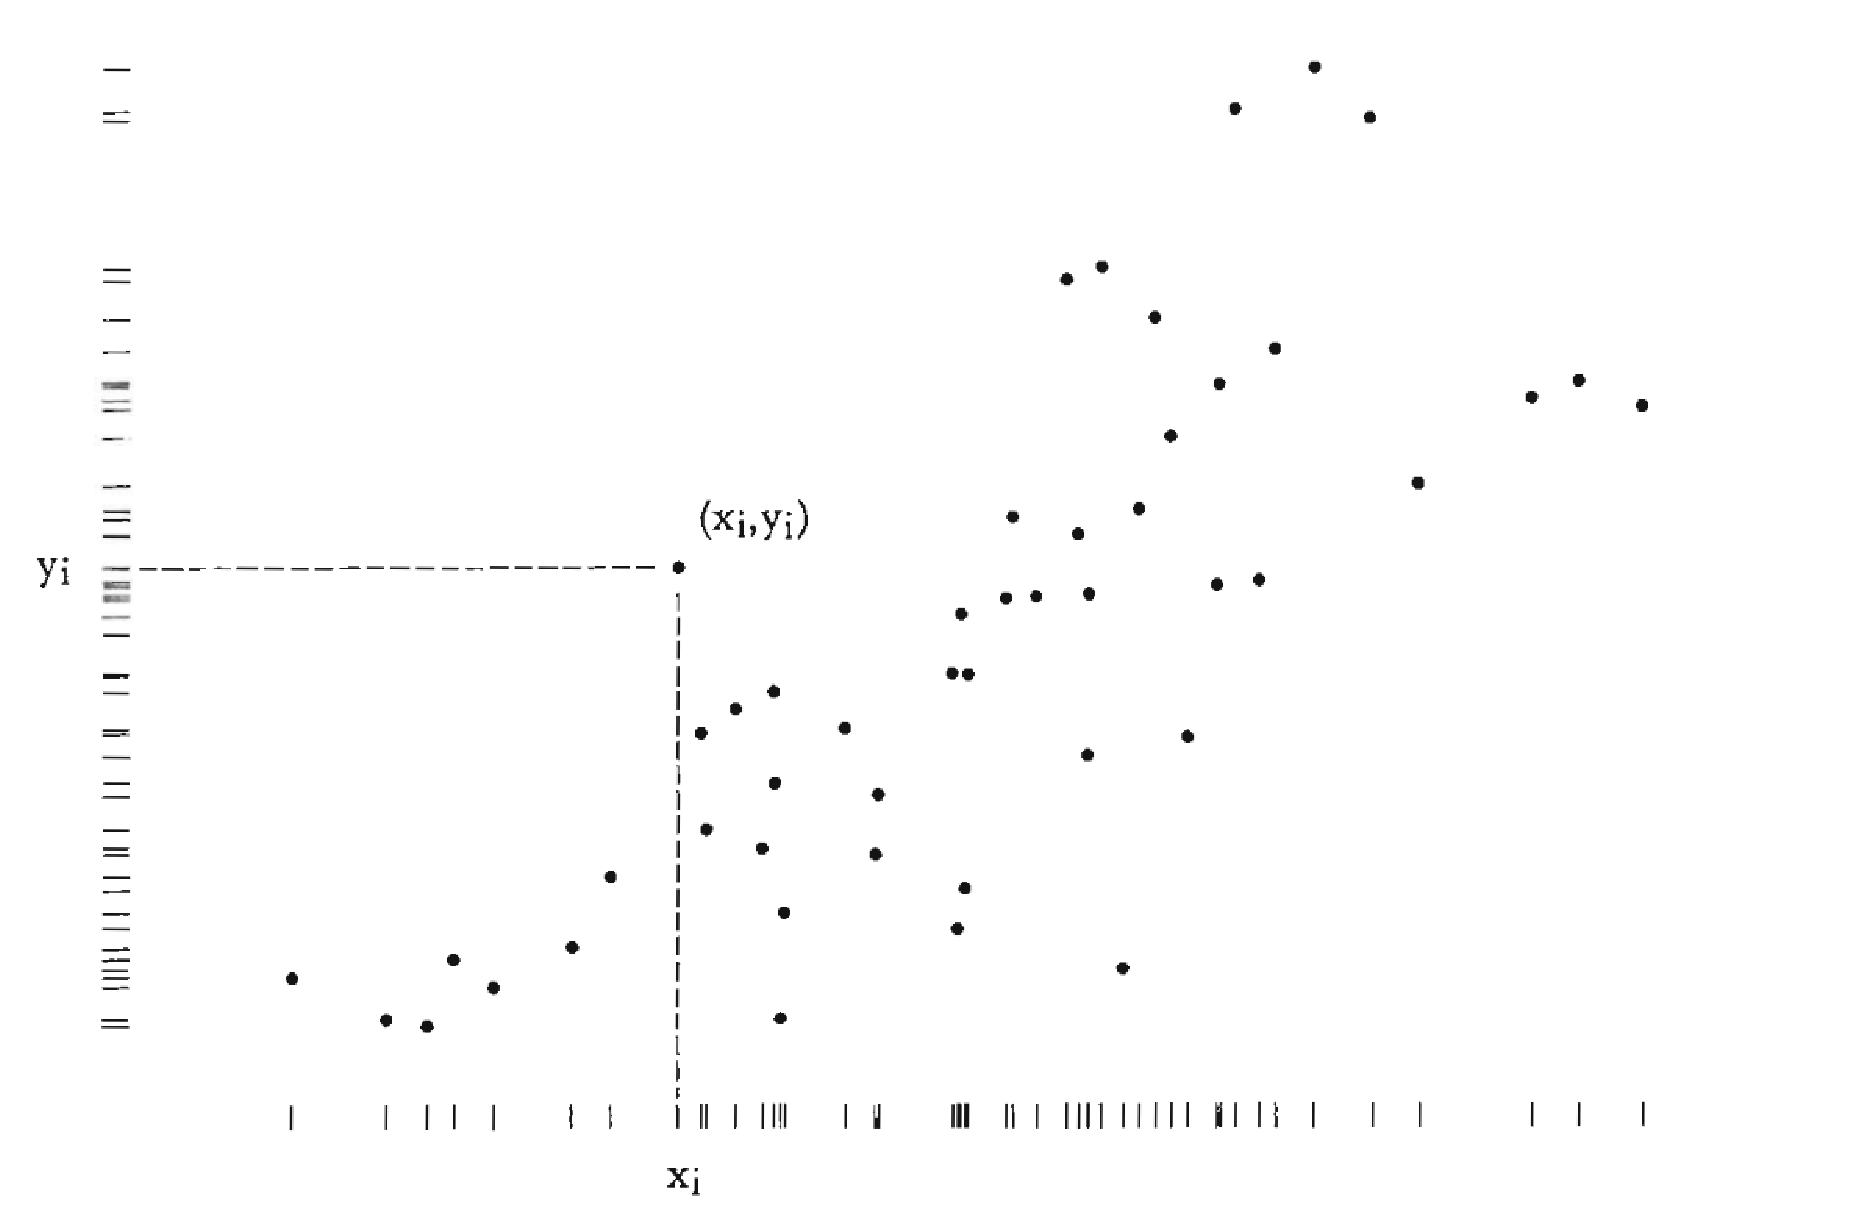
\includegraphics[width=07cm]{./illustrations/annexes/axesdistributions.eps}
}

Ticking is also subjected to improvment : In small set of data, printing actual numbers from the set instead of arbitrary rounded up numbers can also make the axis more efficient.

Effciency in representing data can be found by representing multiple informations with a single point. A point on a map represent the location, the name of a city and can also represent another variable.

%Image des troupes
\centerline{
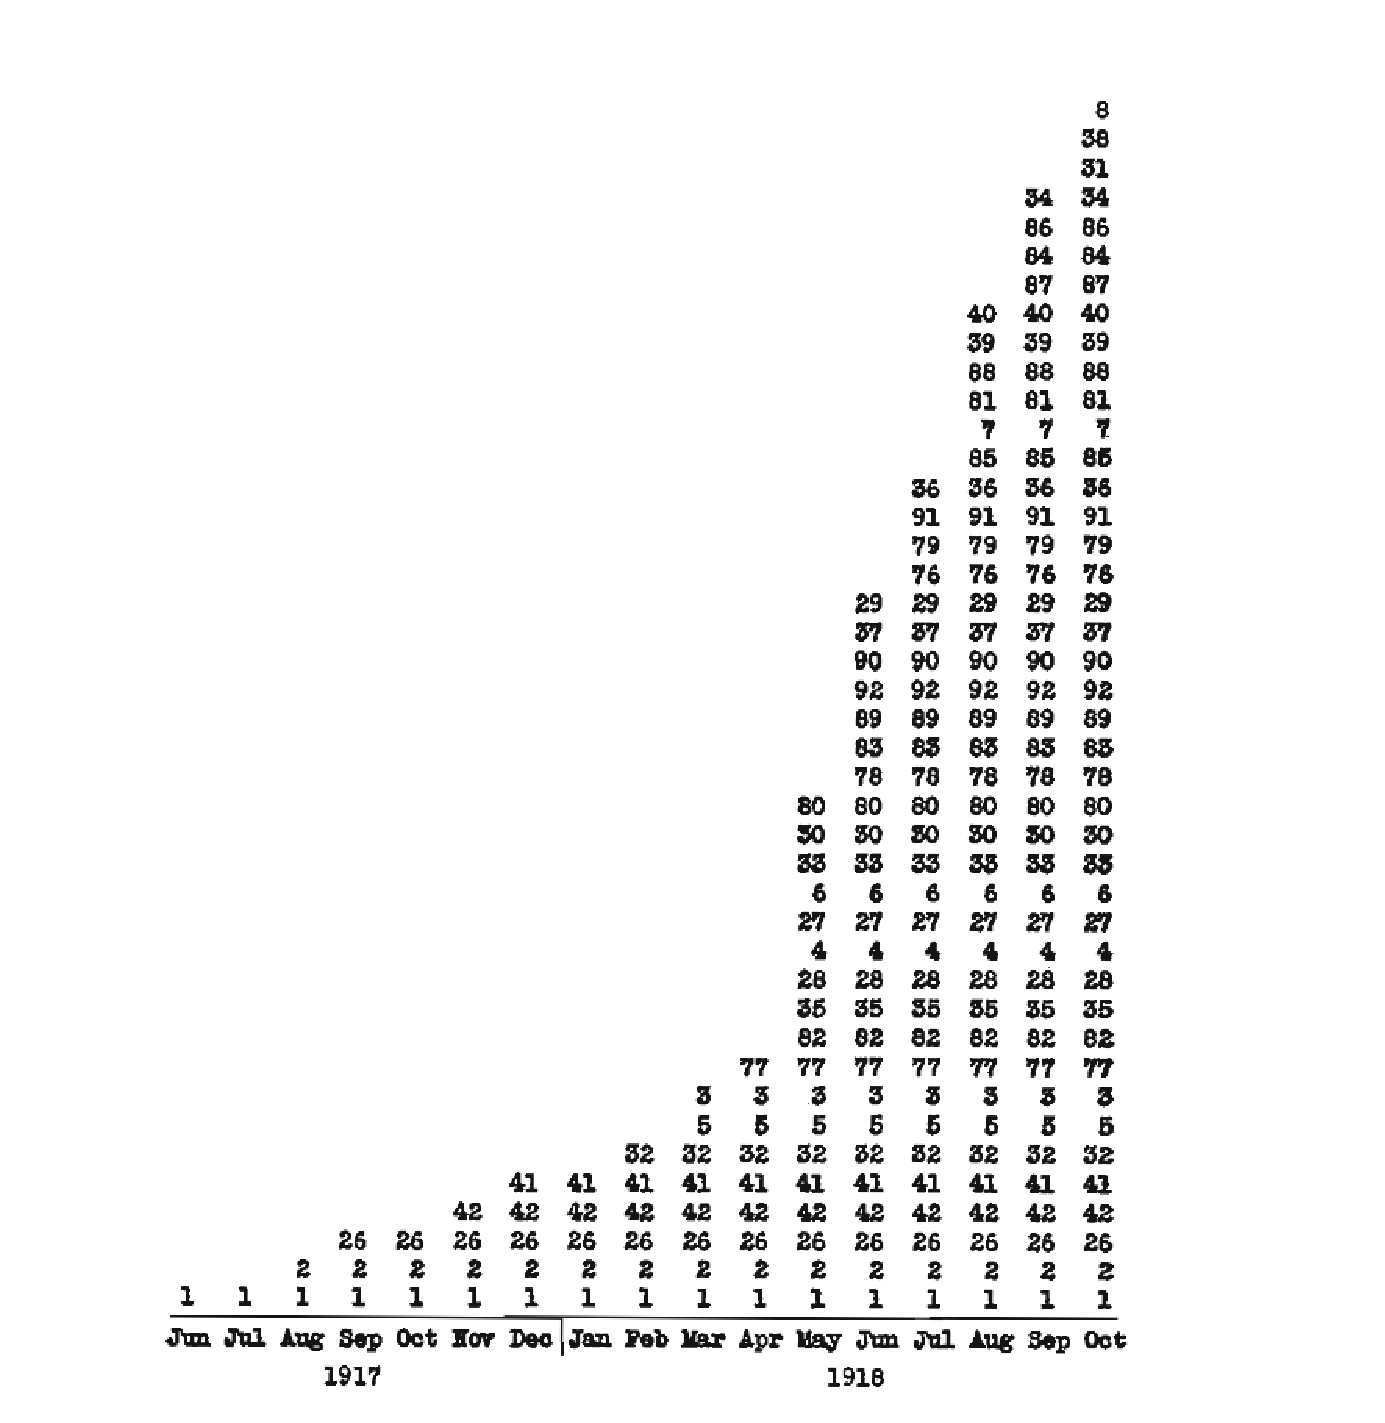
\includegraphics[width=07cm]{./illustrations/annexes/temps_wwi.eps}
}

 Push to its limit, this idea can be very interesting : What if the data was represented by its number ? In short to medium sized data set, this idea can sometime be interesting.
 This chart shows, with the economy of one axis, three informations : 

\begin{itemize}
\item the number of fivision for each month, June 1917 to October 1918
\item what particular division were in France in each month
\item the duration of each division's presence in France
\end{itemize}

%Image p.141
\centerline{
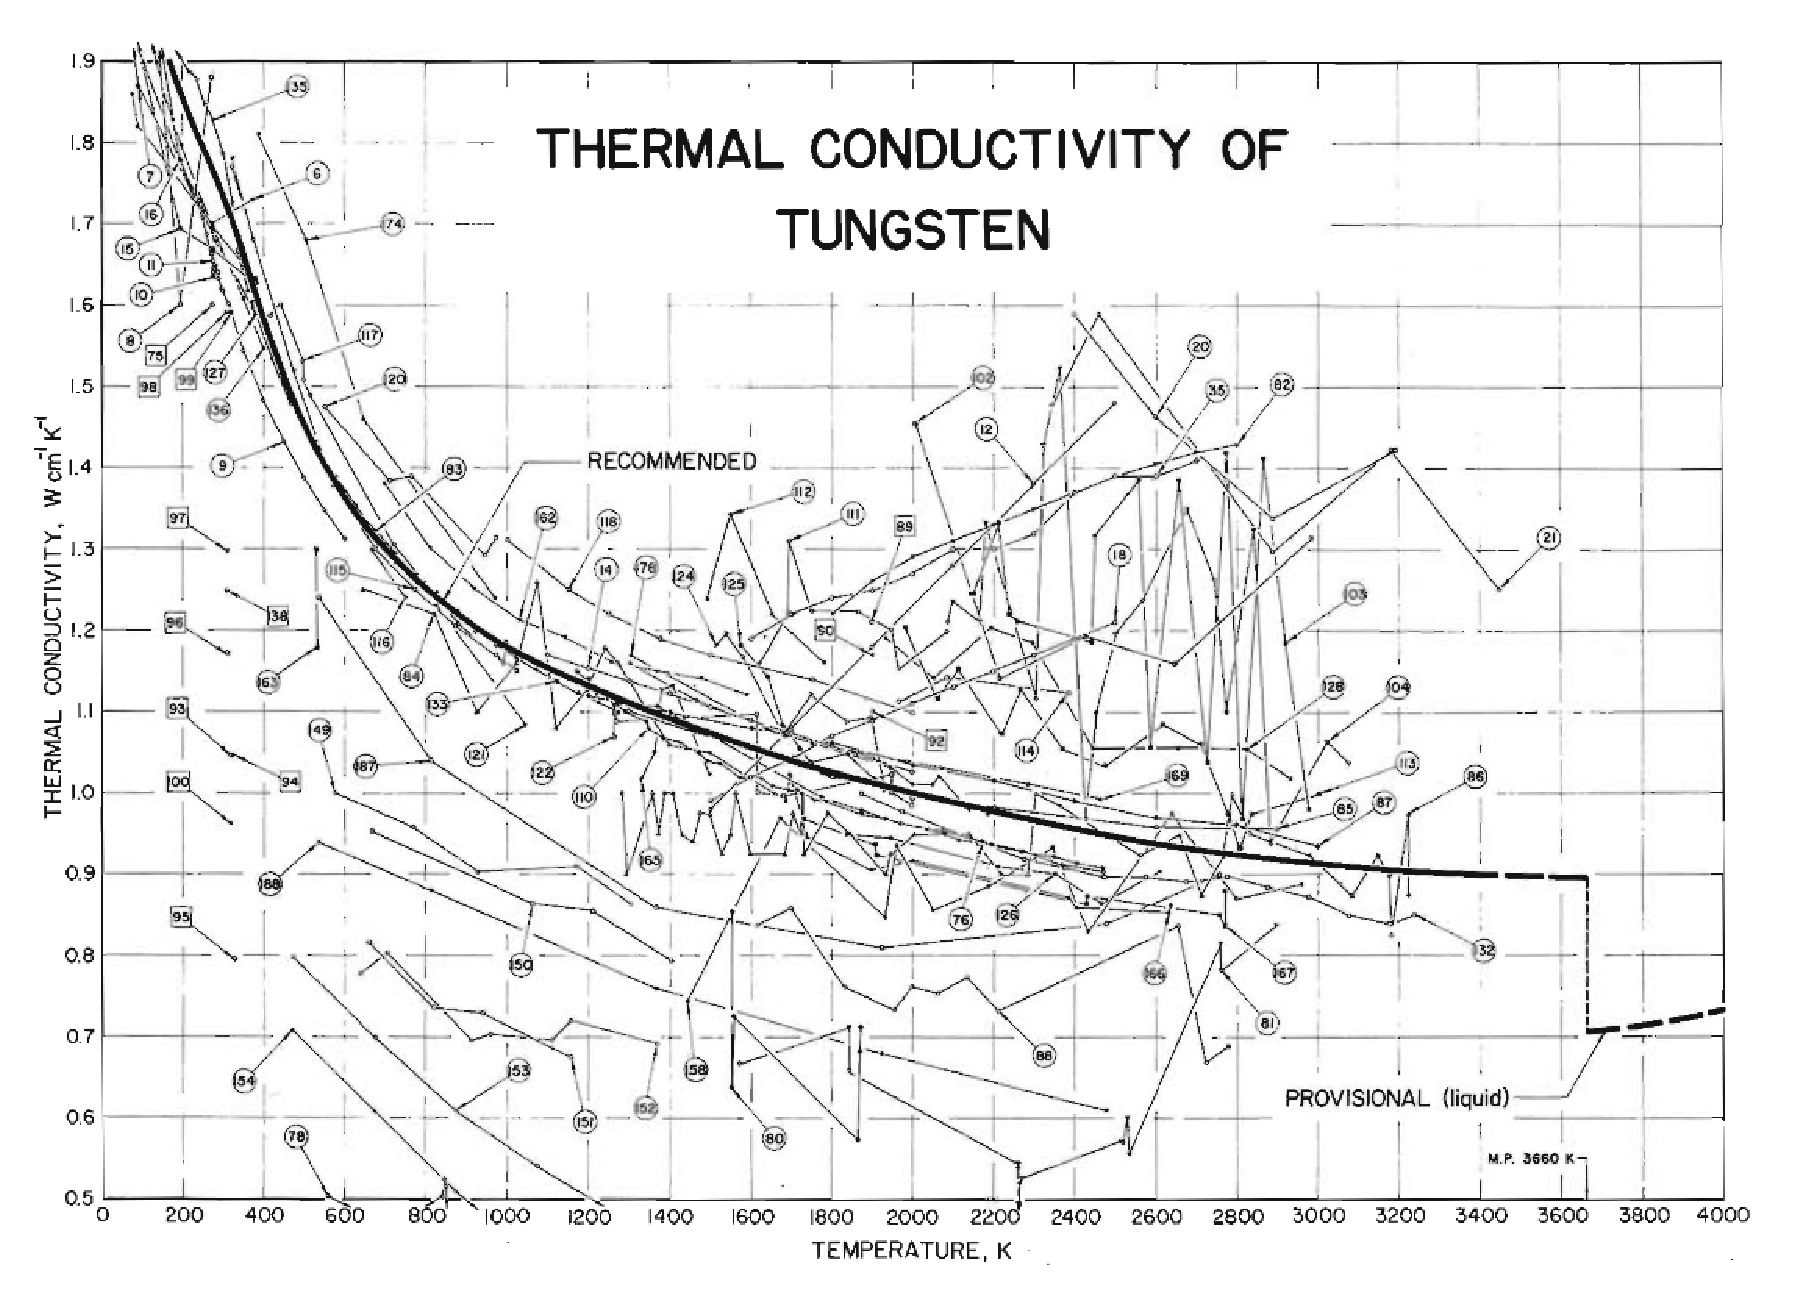
\includegraphics[width=10cm]{./illustrations/annexes/relationel_tungsten.eps}
}
The name given to a data serie can also be interesting if it is chosen wisely.
 If there are a hundread series in a plot, that they are named according to this model : ``61c'' stands for \emph{The third study made in 1961}, and that this name is shown on the plot, it can add a lot of information for the focused viewer.

To judge if a graph is intuitive, the following question should be asked : \emph{Does the viewer see the data or interprate the graphic ? Is my diagram telling a story when glanced at it ? When seen up close, are my data point all making sense ?}
 Color is not often an intuitive medium, for it is not immediately translatable by the viewer in data without jumping to the legend and see what it means. Shade of greys are more efficient. A graphic made of several small graphics can be a very efficient way of showing a lot of data, and compare several states of an object.

Finally, line weight and lettering should be proportional to the importance of what they represent. Not all of the element should thick, nor should all they be thin. A balance shall be found. A rectangle graphic is also always better.
\section{Conclusion}
%Conclusion here written 

The place of graphic in edition have to be rethink. For small sets of data, wordly graphic or table are preferable, since graphic does not improve much their readability. Graphic should be used for a big sets of data. and they be should integrated to text. 
\begin{quote}
Data graphics are paragraphs about data and should be treated as such.
\end{quote}
